%% Document %%
\documentclass[12pt]{book}


%% Packages %%
\usepackage{ucs}
\usepackage[utf8x]{inputenc}
\usepackage[francais]{babel}
%\usepackage{fullpage}
\usepackage{mathpple}  % Pour la police
\usepackage{graphicx}
\usepackage{hyperref}
\usepackage{amsmath}   % Pour numberwithin
\usepackage{tocloft}   % pour cftsecaftersnumb ***
%\usepackage{spacing} \begin{spacing}{0.8} toto \end{spacing}
%\makeatletter \renewcommand{\numwidth}{9.55em plus1fil} \makeatother
\usepackage{fullpage}



%%%%%%%%%%%%%%% Modification de la taille des captions
\newcommand{\captionfonts}{\small\itshape}

\makeatletter  % Allow the use of @ in command names
\long\def\@makecaption#1#2{%
  \vskip\abovecaptionskip
  \sbox\@tempboxa{{\captionfonts #1: #2}}%
  \ifdim \wd\@tempboxa >\hsize
    {\captionfonts #1: #2\par}
  \else
    \hbox to\hsize{\hfil\box\@tempboxa\hfil}%
  \fi
  \vskip\belowcaptionskip}
\makeatother   % Cancel the effect of \makeatletter
%%%%%%%%%%%%%%% Find de la modification


%% Metadata %%
\title{\Huge{Rapport bibliographique}\\\Large{Correction du mouvement respiratoire en TEP}}
\author{
        \vspace{2cm}
        Simon Marache-Francisco \\
        Laboratoire CREATIS/LRMN - Philips Medisys\\
        \vspace{2cm}
}
\date{\today}



%% Data %%
\begin{document}

\addtolength{\parskip}{0.5em}

\numberwithin{section}{part} 
%%%%%%% pour éloigner le texte de la tables des matières des nombres
\renewcommand{\cftsecaftersnumb}{\hspace{1em}}
\renewcommand{\cftsubsecaftersnumb}{\hspace{1em}}
\renewcommand{\cftsubsubsecaftersnumb}{\hspace{1em}}


\newcommand{\verrous}{\textbf{Verrous levés}}

\newcommand{\todo}[1]{
\addcontentsline{toc}{subsection}{\textbf{Todo:} #1}
$\|$\textbf{A Faire : }#1$\|$
}


\maketitle
\thispagestyle{empty}

\begin{center}
	\begin{tabular}{c c}
		
\includegraphics[width=5cm]{images/logoPhilips} & 
\includegraphics[width=5cm]{images/logoCREATIS}
	\end{tabular}
\end{center}


\vfill

\textbf{A destination de :}
\begin{itemize}
    \item Jean-Michel Rouet, Philips Medisys
    \item Carole Lartizien, CREATIS/LRMN
    \item Rémy Prost, CREATIS/LRMN
\end{itemize}
\newpage

\tableofcontents


\part{Introduction}

\part{Imagerie TEP}
	\chapter{Principe Physique}
		\section{Généralités}
		\section{Diffusions}
		\section{Attenuation}

	\chapter{Déroulement d'une acquisition}
		\section{2D / 3D}
		\section{list-mode}

	\chapter{Algorithmes de reconstruction}
		\section{Itératifs}
			\subsection{EM}
			\subsection{OSEM}
		\section{Analytiques}
			
%	\chapter{Imagerie TDM}

\part{Mouvement respiratoire}
%	\chapter{Modalités d'imageries}
%	
\section{Tomographie par émission de positons (PET)}

\subsection{Historique}

\subsection{Principe physique}

\subsection{Reconstruction des images}

\section{Tomodensitométrie}

La tomodensitométrie (TDM) est une technique d'imagerie utilisant les rayons X pour imager l'atténuation des tissus. Ils sont transmis d'une source sur un détecteur à travers le corps humain et renseignent sur les différentes atténuation des tissus présents. Des algorithmes de reconstruction analytiques ou itératifs (fedkampf)


\subsection{Historique}

\subsection{Principe physique}



\subsubsection{Physique}

\subsection{Reconstruction des images}




	\chapter{Respiration et influence sur les acquisitions TEP/TDM}
	Le mouvement respiratoire en imagerie TEP engendre plusieurs effets sur les images reconstruites, qui seront détaillés ci-après. Ils occasionnent notamment une diminution de la qualité des images, ce qui peut perturber le travail des praticiens.

\section{Mouvement respiratoire}

Ce mouvement est la succession d'une phase inspiratoire, suivi d'une phase expiratoire. Chacune de ces phases combine plusieurs mouvements élémentaires~\cite{servant2007cours} :
 
\begin{enumerate}
 \item thoracique, avec un déplacement des côtes
 \item abdominal, avec un déplacement du diaphragme
 \item en cas d'inspiration forcée, action des pectoraux
\end{enumerate}

\begin{figure}[h!]
    \begin{center}
	\begin{tabular}{c c c}
        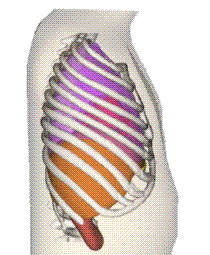
\includegraphics[width=4cm]{images/resp1} & 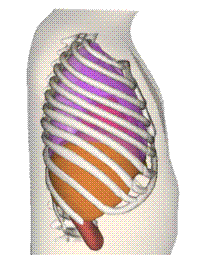
\includegraphics[width=4cm]{images/resp3} & 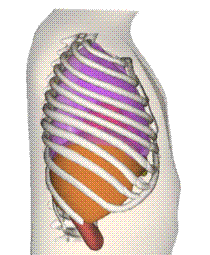
\includegraphics[width=4cm]{images/resp5} \\
	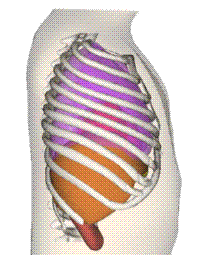
\includegraphics[width=4cm]{images/resp7} & 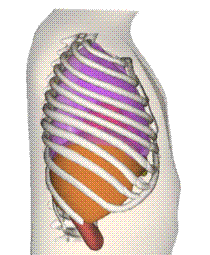
\includegraphics[width=4cm]{images/resp9} & 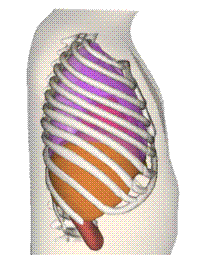
\includegraphics[width=4cm]{images/resp11}\\
	\end{tabular}
    \end{center}
    \caption{Modélisation de la respiration par le fantôme XCAT.}
    \label{fig:respiXCAT}
\end{figure}

La variabilité inter et intra-patient de ce mouvement est très importante : le volume d'air inspiré peut varier de 500mL à 1200mL selon que la personne a une respiration normale ou profonde. Pour ces deux extrêmes, la fréquence respiratoire varie de 5 cycles/min. à 20 cycles/min.~\cite{sherwood2006fundamentals}.

Or une acquisition TEP a une durée de plusieurs minutes par lit, ce qui amène à la reconstruction d'une image dégradée, notamment au niveau de la localisation de la tumeur, de son activité mesurée et, par extension, de sa détection. De le même manière, des artefacts apparaissent au niveau des zones de forts mouvement dans les images TDM, lorsque les organes bougent pendant une rotation du capteur.

Je vais tout d'abord introduire les effets visibles sur les images, puis je m'attarderais sur les mesures quantitatives utilisés pour mesurer l'apport de la correction du mouvement sur les tumeurs. Ensuite, je détaillerais les publications utilisant des critères pouvant être assimilés à de la détection.

\section{Localisation et Volume}

\begin{equation}
\%PRD= \left| \frac{Image~non~corrig\acute{e}e - Image~de~r\acute{e}f\acute{e}rence}{Image~de~r\acute{e}f\acute{e}rence} \right|
\label{eq:PRD}
\end{equation}

La localisation et le volume des tumeurs peuvent être modifiés par le mouvement engendré par la respiration (voir figure \ref{fig:effetMvt}). D'après~\cite{lamare2007respiratory}, réalisé sur des simulations monte-Carlo à l'aide du logiciel de simulation Geant4\cite{jan2004gate} en utilisant le modèle NCAT\cite{segars2001These}, la largeur à mi-hauteur des lésions peut être modifiée de 48\% (equation \ref{eq:PRD} : Percent relative difference) dans le cas d'une lésion de 7mm de diamètre dans la partie basse du poumon. L'imprécision axiale sur le positionnement de la tumeur peut atteindre 9\% dans les mêmes conditions.

\begin{figure}[h!]
    \begin{center}
            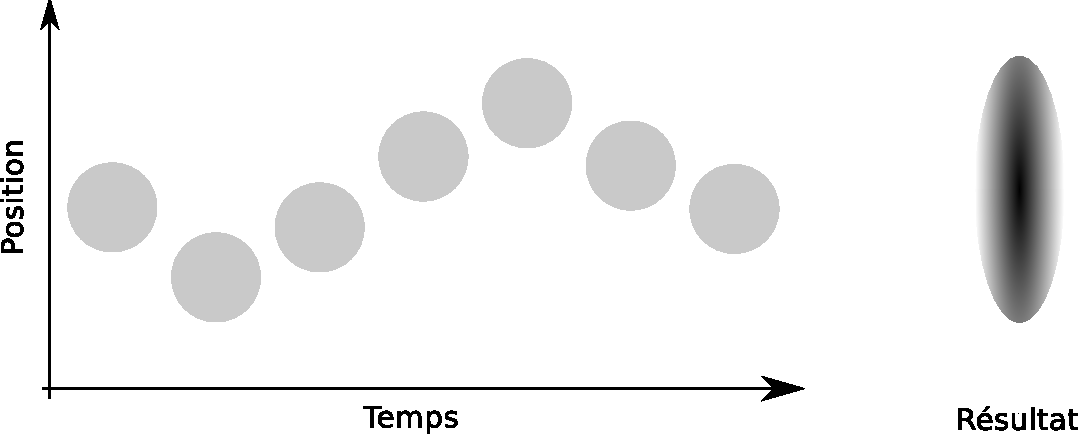
\includegraphics[width=10cm]{images/moyennageImage} \\
    \end{center}
    \caption{Effet du déplacement d'une tumeur sur les données acquises. La position de la tumeur change en fonction du temps, ce qui provoque l'acquisition d'une tumeur équivalente présentée à droite.}
    \label{fig:effetMvt}
\end{figure}


\section{Mesure de l'activité des tumeurs}

Le contraste des tumeurs par rapport au fond est un critère important pour déterminer la malignité des tumeurs~\cite{dimitrakopoulou2002role}~\cite{krak2005effects}. Mais il va aussi directement déterminer si la tumeur est détectable ou non.

L'article de \cite{GuopingChang2010Implementation} est une évaluation clinique réalisée sur 13 patients (21 tumeurs au total).

L'activité peut être influencée par la respiration de deux manières : par un mauvais ajustement de la carte d'atténuation, et par le moyennage de la position de la tumeur.

\subsection{Décalage de la carte d'atténuation}

La carte d'atténuation utilisée pour corriger les images reconstruites est basée sur une image TDM prise à un instant donné du cycle. Or l'atténuation de la zone correspondant à une tumeur peut être différente de celle du tissus environnant.

\begin{equation}
\label{eq:varSUV}
 \%~variation~SUV_{max} = 100 \times \frac{ | SUV_1 - SUV_2 | }{ (SUV_1 + SUV_2) / 2 }
\end{equation}

D'après l'étude~\cite{erdi2004ct} réalisée sur cinq patients, on peut observer des variations de $SUV_{max}$ (voir eq. \ref{eq:varSUV}) allant jusqu'à 24\% selon que la correction d'atténuation est réalisée à partir d'une image TDM en fin d'expiration ou d'inspiration. Sur l'ensemble du cycle, la variation peut atteindre 30\%.


\subsubsection{Artefacts dûs à l'utilisation de l'image TDM}

On peut voir sur les images de la figure \ref{fig:artefactsCT} des artefacts présents sur les images TDM utilisées pour la correction d'atténuation. Ces artefacts proviennent de la manière dont les images sont acquises : la caméra tourne autour du sujet dans un mouvement hélicoïdal, et l'algorithme de reconstruction va ensuite utiliser les acquisitions pour reconstruire une image complète. Or en cas de respiration rapide, des incohérences peuvent survenir quand le mouvement du diaphragme est tellement rapide qu'il va plus vite que la caméra. Ce type d'artefacts va créer des incohérences dans les images TEP reconstruites.

\begin{figure}[h!]
	\begin{center}
		\begin{tabular}{c c}
			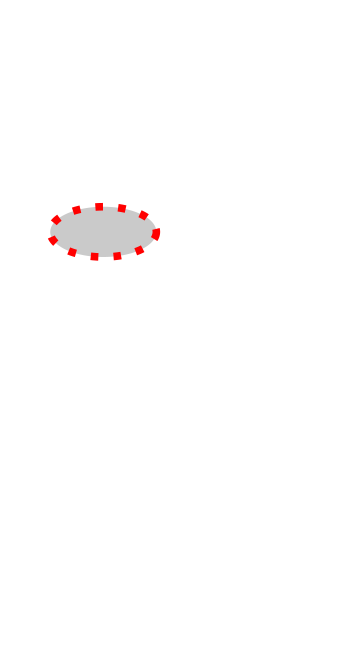
\includegraphics[width=5cm]{images/artefactCT1} & 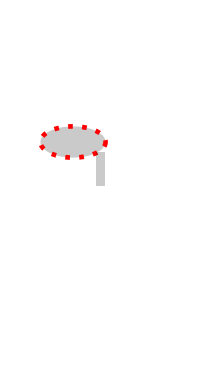
\includegraphics[width=5cm]{images/artefactCT2}
		\end{tabular}
	\end{center}
	\caption{Artefacts présents sur des images TDM utilisées pour la correction d'atténuation} 
	\label{fig:artefactsCT}
\end{figure}


\subsection{Déplacement de la tumeur au cours du cycle}

Le mouvement respiratoire va avoir pour effet de déplacer la tumeur pendant l'acquisition, ce qui va moyenner la quantité de radioactivité sur l'ensemble du cycle. Si le déplacement de la tumeur est suffisamment grand par rapport à son diamètre, la réduction de radioactivité va être importante.

L'étude \cite{boucher2004respiratory} montre que sur des fantomes, un déplacement d'une source radioactive de 6mm sur un cycle respiratoire moyen entraîne une sous-estimation de l'activité maximale de la tumeur de 41\% pour une lésion de 1.2mL et de 21\% pour une sphère de 19.4mL.


\section{Impact du mouvement respiratoire sur la detection}

Peu de travaux ont été réalisés sur l'impact du mouvement respiratoire sur la détection des tumeurs. Globalement, les critères utilisés sont principalement des mesures orientées sur quantification des lesions ($SUV_{max}$, profils de lesions, ...). Très peu d'articles utilisent des critères orientés détection tels que les observateurs.

Voici une liste des critères utilisés dans différentes publications pour évaluer la performances d'algorithmes de correction du mouvement respiratoire :

\begin{enumerate}
 \item  $SUV_{max}$, contraste : \cite{GuopingChang2010Implementation} \cite{lamare2007list} \cite{nehmeh2002effect} \cite{detorie2008quantitative}
 \item Line profile : \cite{GuopingChangImplementation} \cite{Thielemans2006Lesion} \cite{lamare2007list}
 \item Volume et position de la lésion : \cite{GuopingChangImplementation} \cite{lamare2007list} \cite{nehmeh2002effect}
 \item Rapport signal sur bruit (SNR) : \cite{GuopingChangImplementation}
 \item Observateur de Hotelling (CHO) : \cite{Thielemans2006Lesion}
\end{enumerate}

Comme on peut le voir, les deux seuls critères qui pourrait s'approcher d'une étude sur la détection sont le SNR et le CHO, mais ils sont largement sous-représentés. 

Je vais me concentrer sur les deux publications qui utilisent un observateur, et présenterai les résultats des autres publications dans la partie suivante.

Un autre document par rahmim arman~\cite{rahmim4d} propose d'utiliser le CHO pour évaluer l'amélioration de la détection des défauts dans de l'imagerie cardiaque corrigée du mouvement respiratoire. Ce document n'a pas encore donné lieu à publication.

\subsection{Thielemans 2006}

Dans sa publication, Thielemans~\cite{Thielemans2006Lesion} utilise le CHO~\cite{barrett1993model} dans le cas ou le signal (activité des lesions) et le fond sont connus (activité du poumon). Cet observateur est un classifieur linéaire, utilisé en conjonction avec des informations fréquentielles. 

Cependant ils utilisent le CHO uniquement sur des lésions de fort diamètre et contraste (13mm de diamètre et contraste de 4.25:1, sur des simulations analytiques). Les résultats présentés (fig. \ref{fig:apportCHO}) montrent une amélioration du score pour les méthodes de correction de l'ordre de 50\% dans certains cas. 

Mais il est difficile d'évaluer de manière précise l'apport des méthodes de détection à l'aide de ces seuls ``scores'' car ce sont des résultats qualitatifs. 

\begin{figure}[h!]
	\begin{center}
		\begin{tabular}{c c}
			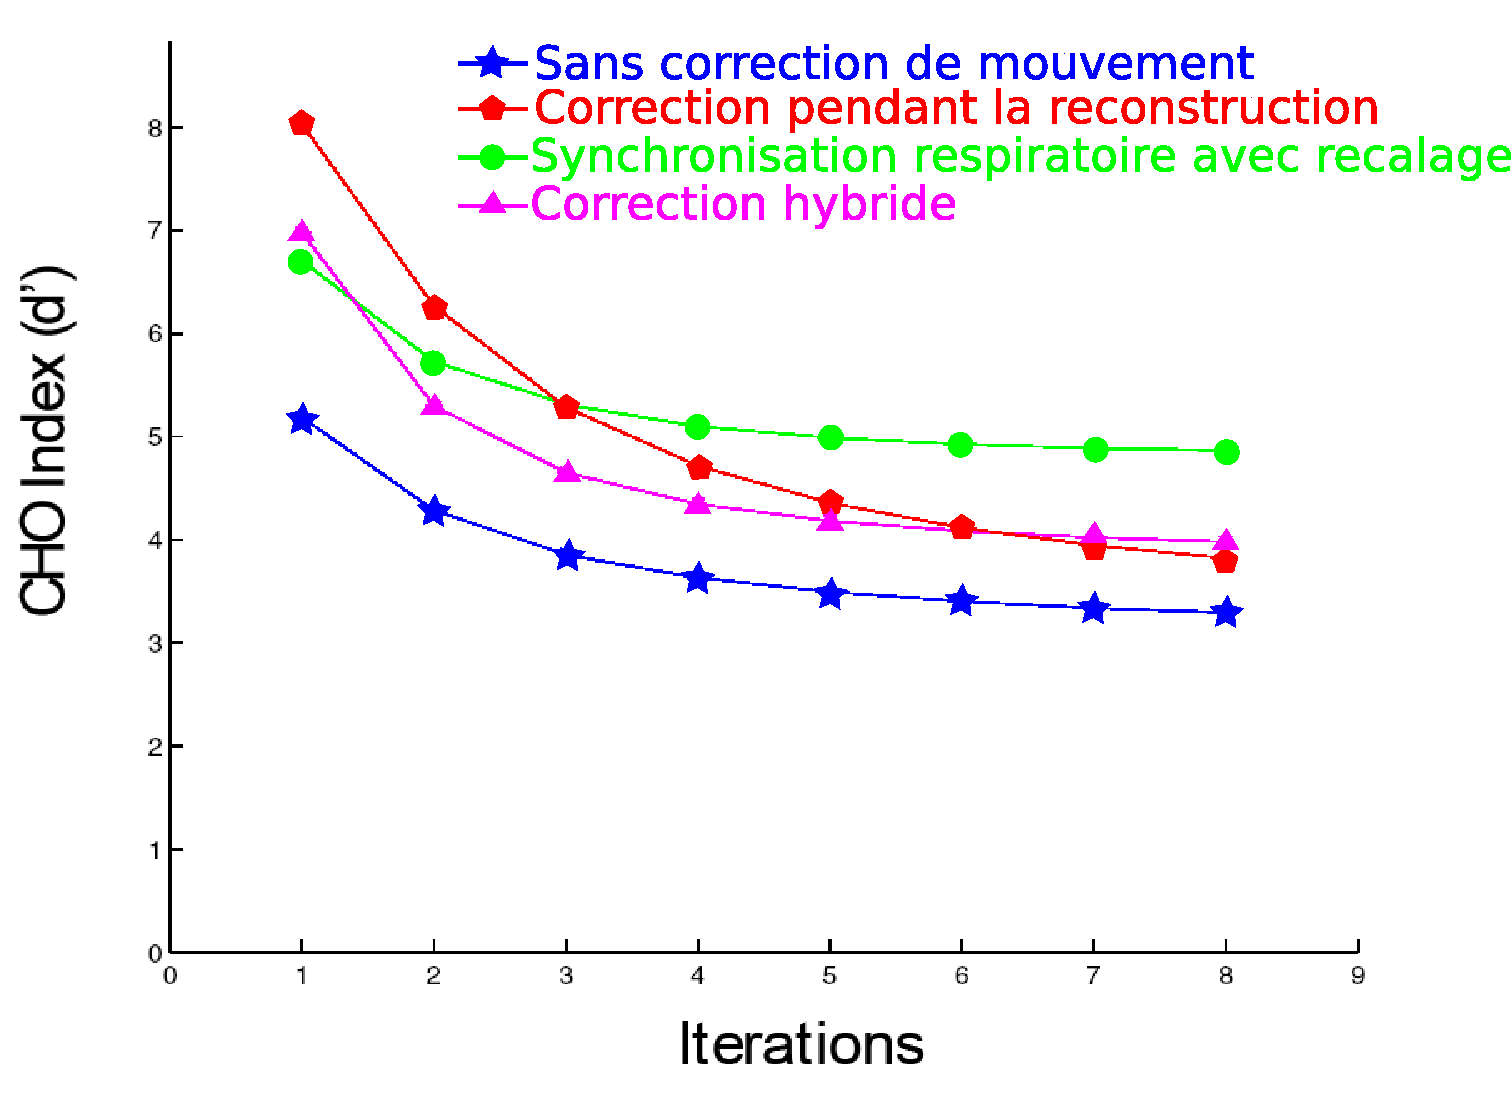
\includegraphics[width=10cm]{images/apportCHO}
		\end{tabular}
	\end{center}
	\caption{Index de CHO pour différents techniques de correction du mouvement respiratoire en fonction du nombre d'itérations. la méthode utilisant le gating est comparée avec une méthode évolution présentée dans le document.} 
	\label{fig:apportCHO}
\end{figure}


\subsection{Chang 2010}

Cette publication utilise entre autres le rapport signal sur bruit pour évaluer l'amélioration de la visibilité des lésions. Son interêt est qu'elle est réalisée sur 13 patients et compare les performances sur 21 tumeurs au total.

Ils ont calculés le rapport signal sur bruit (SNR) en divisant le SUV moyen de la tumeur par l'écart-type d'une zone d'interêt dans le poumon. On observe une amélioration moyenne de 26\% du SNR sur les tumeurs, et pouvant atteindre 66\%.

Il est intéressant de constater qu'il y a un point où le SNR diminue de 3.4\%, mais que le $SUV_{max}$ et le $SUV_{moyen}$ augmentent tout de même de presque 18\%. Cela semble indiquer une erreur car le SUV de la zone d'interêt n'est pas censé changer de manière importante.

	
	\chapter{Processus d'estimation du mouvement}
	\section{Estimation du signal respiratoire}

Le signal respiratoire est une grandeur qui permet de positionner le cycle entre la fin d'inspiration et la fin d'expiration. Il est habituellement fourni par des capteurs externes qui génèrent un signal qui sera corrélé avec la respiration. Cela permet de faire correspondre les données acquises par un imageur avec une phase particulière du mouvement respiratoire.

\subsection{Spiromètre}

Le spiromètre est un capteur externe placé sur la bouche du patient et qui permet de mesurer les déplacements d'air dans le système respiratoire~\cite{guivarc2004synchronization}. Les spiromètres mesurent un débit ou un volume d'air inspiré/expiré (voir illustration figure \ref{fig:spirometre}). A partir de l'une des grandeurs, il est possible d'estimer l'autre facilement. L'avantage du spiromètre est qu'il permet d'accéder à une mesure caractérisant directement la respiration du patient, et n'est pas sujet à des perturbations externes (mouvements involontaires par exemple). Par contre cela demande un appareillage qui peut être assez invasif pour le patient.

\begin{figure}[h!]
	\begin{center}
		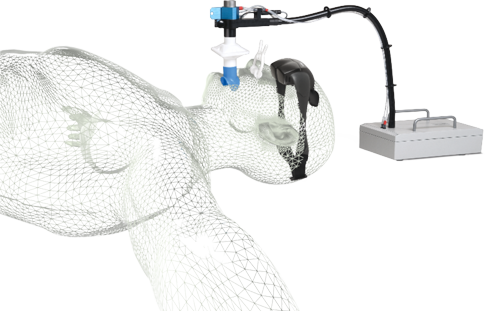
\includegraphics[width=12cm]{images/spiro}
	\end{center}
	\caption{spiromètre Syn'r : on peut voir le système de mesure de la respiration ainsi qu'un système de moniteurs implantés dans les lunettes pour aider le patient à contrôler sa respiration} 
	\label{fig:spirometre}
\end{figure}

\subsection{Ceinture}

Pour mesurer le signal respiratoire, il est possible d'utiliser un capteur qui va mesurer le périmètre du thorax. L'extension de cette ceinture va correspondre aux mouvements de la cage thoracique et de l'abdomen pendant la respiration du patient. C'est une mesure indirecte de l'amplitude du mouvement respiratoire utilisée couramment en routine clinique. 

Différentes technologies existent pour mesurer cette information (RespiTrace R250 de Studley. Data Systems, Respiratory Belt Transducer de ADInstruments, ...). Elles sont basées sur plusieurs effets (résisitif, inductif...) et ont l'avantage d'avoir un faible coût et de ne pas perturber le patient.

Bien qu'elles puissent être influencées par les mouvements involontaires du patient, il a été montré dans \cite{Guivarch2004Sync} que les données acquises selon les méthodes par respiromètre et par ceinture sont équivalentes.

\subsection{Basés caméras}

Des caméras peuvent être utilisées pour estimer le mouvement respiratoire. Une des techniques consiste à utiliser des informations surfaciques en reconstruisant en 3D certaines parties du corps à l'aide de plusieurs caméras (avec ou sans marqueurs) ou de caméra temps de vol. Cela permet d'avoir plus d'informations sur la respiration.

Une autre technique consiste à installer un marqueur sur le corps du patient et de relever les déplacements de ce marqueur sur plusieurs axes à l'aide d'une caméra. Un tel système est décris dans~\cite{nehmeh2002effect} : Respiratory Gating System de Varian Medical Systems (voir figure \ref{fig:RGSdeVarian}).

\begin{figure}[h!]
	\begin{center}
		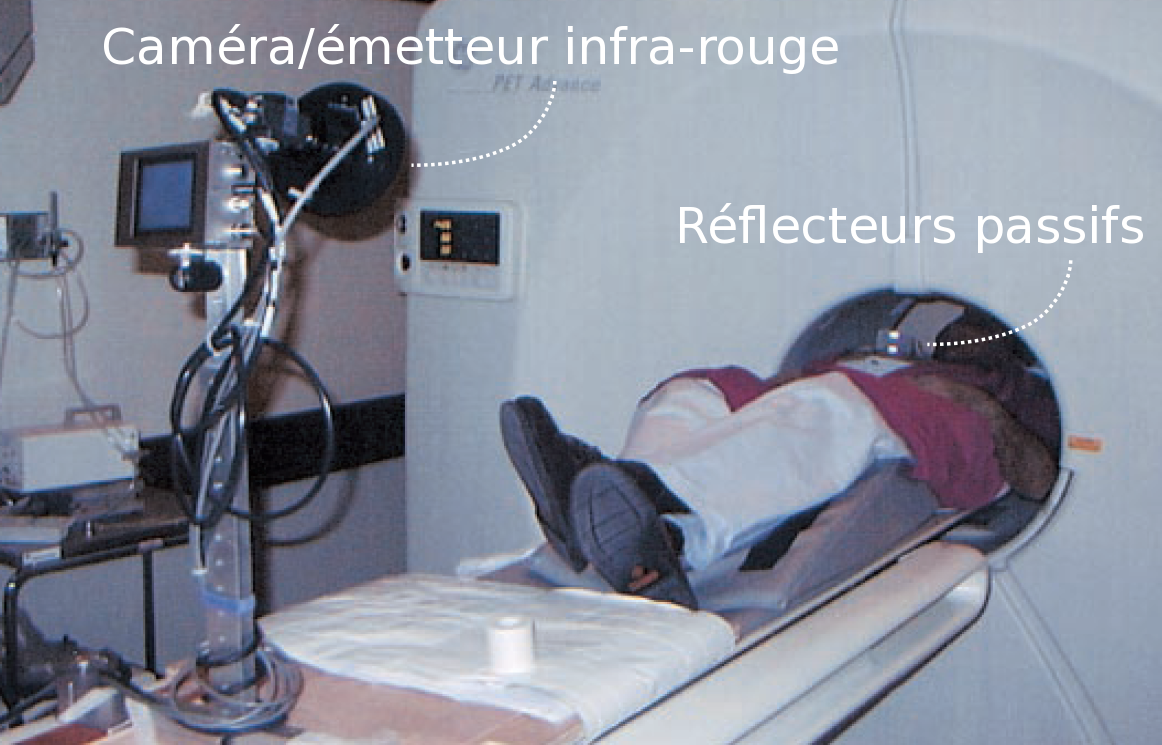
\includegraphics[width=12cm]{images/varian}
	\end{center}
	\caption{Photographie du système RGS de Varian medical Systems en action : une caméra va détecter le déplacement d'une zone du thorax en mesurant le déplacement de marqueurs placés sur un bloc plastique.} 
	\label{fig:RGSdeVarian}
\end{figure}

Ces techniques ont l'avantage d'être moins invasives et plus facilement acceptées par le patient. Cependant, elles sont beaucoup plus sensibles aux mouvements involontaires du patient. Pour l'acquisition d'image TDM ce risque est faible car elles sont de faible durée (inférieures à la minute), mais il devient important pour les acquisitions TEP qui peuvent durer en tout plusieurs dizaine de minutes. Ces mouvements n'étant probablement pas corrélés avec le mouvement respiratoire, ils vont perturber le signal obtenu. 

\subsection{Techniques basées sur les images TEP}
\label{lab:estimMvtTEP}
En TEP, la publication de Bundschuh et al.~\cite{bundschuh2007postacquisition} utilise les données dynamiques pour estimer le signal respiratoire sans avoir besoin de capteur externes . Ce processus est réalisé en 5 étapes : 

\begin{enumerate}
 \item Les données TEP sont acquises en mode séquentiel : toutes les désintégrations détectées sont enregistrées dans un fichier de manière séquentielle  
 \item L'image TEP statique est reconstruite. Elle permet de localiser une lésion dans l'image qui servira d'amer pour l'estimation du mouvement respiratoire.
 \item Une image TEP est reconstruite pour chaque intervalle temporel de 0.5 secondes.
 \item La zone d'intérêt sélectionnée précédemment est sélectionnée dans chaque image reconstruite. La position axiale du barycentre à chaque instant temporel va donner une estimation du mouvement respiratoire pour le volume donné.
\end{enumerate}

Cette technique a été évaluée sur 10 patients et les signaux ont été comparés avec ceux obtenus avec des ceintures abdominales. Pour 3 patients, les courbes respiratoires obtenues par les deux techniques étaient très fortement corrélées. Pour deux autres patients, l'estimation de mouvement obtenue par la TEP était trop bruitée, mais montrait une bonne corrélation avec le signal obtenu par les ceintures abdominales après filtrage. Pour 3 autres patients, il n'a pas été possible de trouver une corrélation entre les deux signaux. Les deux derniers patients ont bougés pendant l'acquisition TEP, ce qui a perturbé le signal.

Cette technique est intéressante mais contrainte par la qualité de l'image TEP. En pratique, la moitié des acquisitions de signaux n'ont pas permis d'obtenir un signal satisfaisant.


\section{Estimation du champ de mouvement}
\label{lab:estimChamp}
Le champ de mouvement est une information beaucoup plus riche que le signal respiratoire car il permet de suivre les déplacements des organes et des lésions à l'intérieur du corps du patient à l'intérieur d'un cycle respiratoire.

Le signal respiratoire acquis par les méthodes précédemment cités est utilisé pour décomposer les données acquises en TDM ou TEP en plusieurs phases, chacune correspondant à un instant du cycle. Ces informations sont utilisées pour assembler les données acquises pour chaque phase, reconstruites indépendamment. Ces reconstructions vont être utilisées pour estimer le champ de mouvements à l'aide de techniques de recalage.


\subsection{Image TEP 4D}

L'estimation du champ de mouvement respiratoire peut être fait à partir des données TEP, comme il a été montré par \cite{dawood2008respiratory, dawood2006lung}. 

Les techniques utilisées sont analogues à celle présentée en \ref{lab:estimMvtTEP}. Elles consistent à réaliser une acquisition list-mode des données en même temps qu'une acquisition du signal respiratoire, puis à réorganiser les données acquises pour reconstruire les différents instants du cycle indépendamment et sans correction d'atténuation. Le mouvement sera estimé à partir de ces images.

La publication de \cite{dawood2008respiratory} cherche à corriger le mouvement respiratoire, et pour cela fait une estimation préliminaire de ce mouvement. 

Pour obtenir le signal respiratoire, dawood utilise une caméra qui enregistre le mouvement d'un marqueur placé sur l'abdomen du patient. Ce marqueur est un point blanc placé sur un disque noir, et sa position axiale est détectée par seuillage. 

La synchronisation avec l'acquisition PET est réalisée à l'aide d'une LED dans le champ de vue de la caméra qui s'allume lors du début de l'acquisition. Une fois l'acquisition réalisée, le signal respiratoire obtenu est utilisé pour répartir les évènements acquis par l'imageur sur un seul cycle respiratoire. Ce cycle est décomposé en 8 parties qui seront reconstruites séparément, sans correction d'atténuation. 

Les auteurs utilisent ensuite un algorithme de flux optique 3D présenté dans \cite{dawood2006lung} et \cite{horn1981determining} pour déterminer le champ de mouvement : Ils estiment un déplacement entre chaque image du cycle et l'image de référence (la 4è dans le cas de cet article). Le résultat de l'algorithme sera donc une séquence de champ de mouvement formant un champ de déformation 4D.

L'algorithme a été testé sur le fantôme XCAT ainsi que sur les données de 16 patients. La performance de l'estimation de mouvement a été évaluée selon trois critères, évalués sur les images corrigées : la correction du déplacement axial du coeur, le coefficient de corrélation des images corrigées du mouvement, ainsi que le bruit obtenu. Je présenterais ces résultats dans la présentation de cet article dans la partie \ref{lab:correctionDawood2008}.

Bai a présenté une technique d'estimation semblable~\cite{bai2009regularized}. Le principe est le même que pour la publication précédente, mais en réalisant une estimation du mouvement à l'aide de B-splines~\cite{thevenaz2000optimization}.

Un exemple de champ de déformation obtenu est présenté en \ref{fig:champMouvementBai}

\begin{figure}[h!]
	\begin{center}
		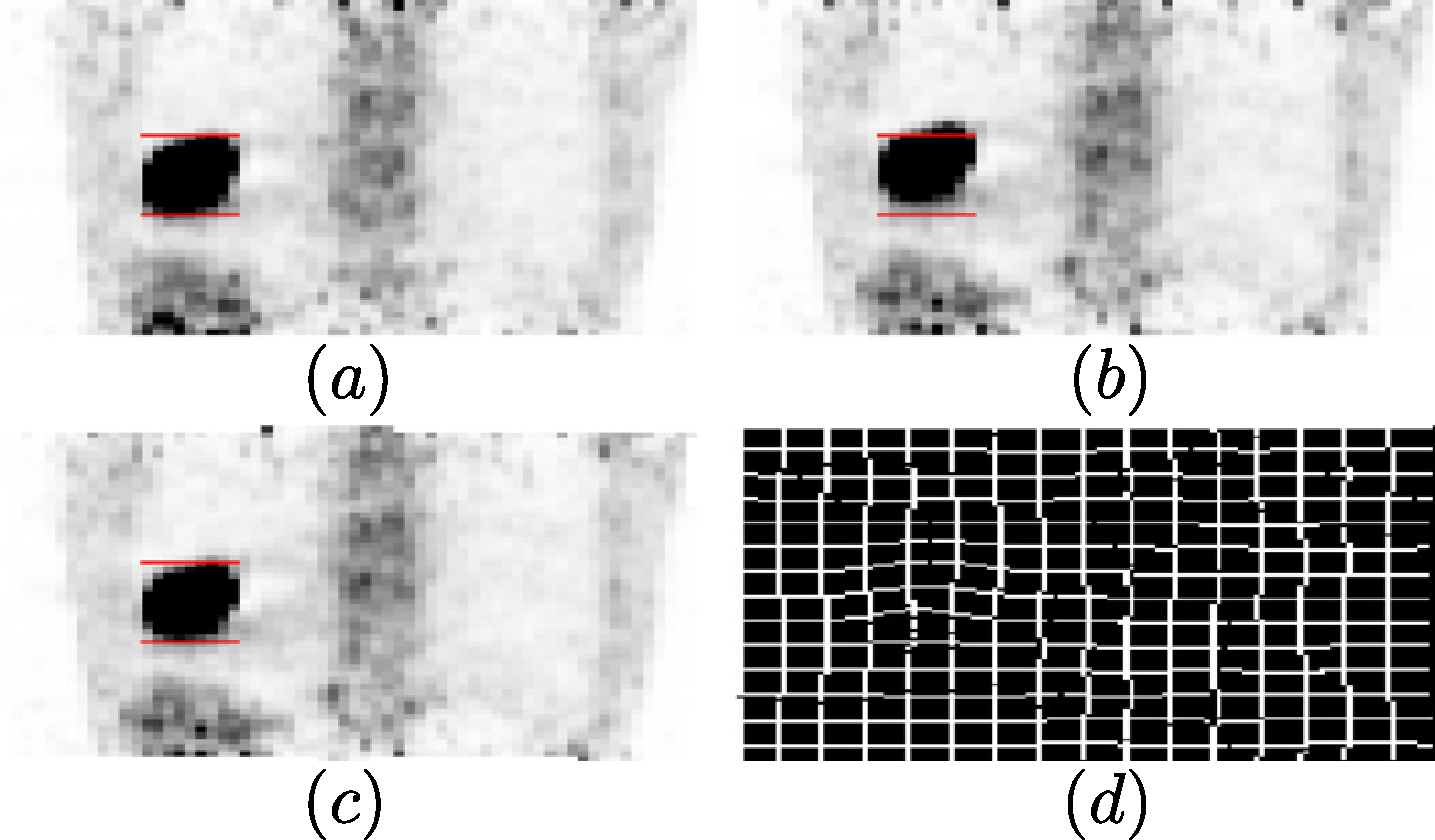
\includegraphics[width=12cm]{images/champDeformBai2}
	\end{center}
	\caption{Champ de déformation calculé à l'aide de la méthode présenté en \cite{bai2009regularized}. a) représente l'image TEP obtenue à partir des données de la phase de référence  (mi-expiration), b) correspond à l'image reconstruite pour les donnée d'expiration complète, et c) le résultat du recalage de l'image de fin d'expiration sur l'image de référence. d) représente le champ de mouvement résultat. Les traits rouges représentent l'extension axiale de la tumeur dans l'image de référence.} 
	\label{fig:champMouvementBai}
\end{figure}

\subsection{Image TDM 4D}

Les images TDM peuvent être acquises en mode dynamique de manière à obtenir une suite d'images couvrant tout le cycle respiratoire \cite{lamare2007list, qiao2006motion}. Les données sont reconstruites indépendamment, avec un rapport sur bruit plus faible que sur l'image originale. 

Des algorithmes de recalage sont utilisés de manière à déduire le champ de mouvement. Le principal avantage de l'utilisation des images TDM 4D est la précision des images. En effet, alors que les images TEP ont une résolution de l'ordre de 5mm, les images TDM atteignent des résolutions inférieures au mm, ce qui permet d'obtenir un champ de mouvement beaucoup plus précis. Cependant, utiliser des images TDM 4D a plusieurs inconvénients :

\begin{itemize}
 \item Une possible incohérence entre le cycle acquis en TDM 4D et la respiration du patient en TEP. Bien que les imageurs TEP/TDM couplent les deux imageurs sur la même machine, de manière à éviter les mouvements du patients entre les acquisitions, le cycle acquis en TDM ne représente qu'un cycle, tandis que l'acquisition TEP va donner un ``cycle moyen`` plus proche de la réalité.
 \item Une dose de radiation émise plus importante. Bien que les technologies récentes permettent de réduire les doses de manière importante pour l'acquisition dynamique, elles restent tout de même plus importantes que pour un CT 3D.
\end{itemize}

Il faut noter que plusieurs publications basées sur des simulations se servent des cartes de labels utilisées pour la simulation pour réaliser les estimation de mouvements~\cite{lamare2007list}. Cela donne une estimation dans le ``meilleur des cas'', où l'image TDM est parfaitement en phase avec les images TEP.

\section{Modèle}

Une autre voie est en cours de développement basée sur la création d'un modèle de respiration qui est adapté à chaque patient à partir d'une quantité réduite de données. Fayad \cite{fayad2010application} propose un modèle basée sur l'analyse en composantes principales. 

Ce modèle est adapté à un patient à partir de deux images TDM prises à des instants différents du cycle, et d'un maillage dynamique de la surface du corps du patient obtenue pendant un cycle respiratoire complet. Dans son implémentation, le maillage est obtenu à l'aide d'une caméra temps de vol.

L'avantage de ce modèle est qu'il est totalement continu, et permet l'extraction d'un nombre arbitraire de phases sous la forme de matrices de déformation. Ce modèle a été testé sur des images simulées (2 fantômes XCAT) et 6 patients.

	
	\chapter{Correction du mouvement respiratoire}
	\label{lab:corrMvt}

\section{Introduction}

Nous allons maintenant présenter les techniques de correction du mouvement respiratoire présentées dans la littérature. 

Deux approches existent pour la correction du mouvement : les techniques dites prospectives, qui consistent à réaliser la correction pendant l'acquisition en sélectionnant les données à conserver, et rétrospectives, qui réalisent la correction à posteriori, après l'acquisition des données. Actuellement, les techniques les plus prometteuses sont rétrospectives, car elles permettent d'utiliser l'ensemble des données du cycle respiratoire.

\section{Synchronisation respiratoire}

La synchronisation respiratoire correspond à un découpage du cycle respiratoire selon la phase (voir Fig.\ref{fig:gatingRespi}) ou l'amplitude (voir figure \ref{fig:gatingRespiAmplitude}). Une seule des phases ou amplitude sera sélectionnée pour la reconstruction. En théorie cela permet d'avoir le meilleur résultat, car il est possible de sélectionner les évènements correspondants à la phase ou l'amplitude où a été acquise la carte d'atténuation.


\begin{figure}[h!]
	\begin{center}
		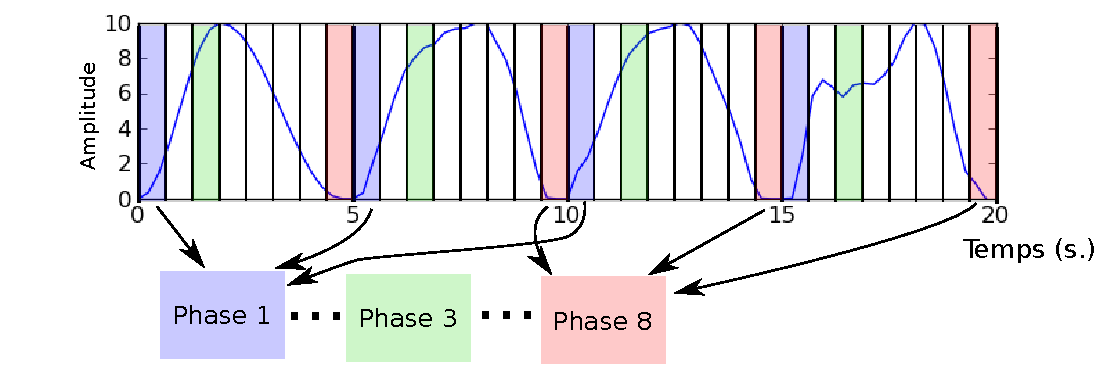
\includegraphics[width=12cm]{images/ET-IM}
	\end{center}
	\caption{Illustration de la synchronisation respiratoire en phase : Le cycle respiratoire acquis est découpé selon la position du signal acquis dans le cycle. Le signal est analysé pour déterminer les débuts et fins de cycles. Chaque cycle est découpé en un nombre déterminé de phases égales.} 
	\label{fig:gatingRespi}
\end{figure}


\begin{figure}[h!]
	\begin{center}
		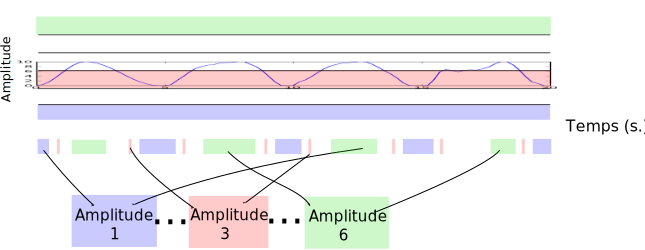
\includegraphics[width=12cm]{images/gatingAmplitude}
	\end{center}
	\caption{Illustration de la synchronisation respiratoire en amplitude : Le cycle respiratoire acquis est découpé selon son amplitude.} 
	\label{fig:gatingRespiAmplitude}
\end{figure}


Cette technique est notamment présentée dans~\cite{nehmeh2002effect}, où le signal respiratoire est estimé par une caméra qui suit un marqueur placé sur le torse du patient (système RPM de Varian Medical Systems). L'étude a été réalisée sur 5 patients volontaires comme suit : un scan de transmission de 3 minutes, suivi d'une acquisition avec correction de 10 minutes, puis d'une acquisition témoin non corrigée de 3 minutes. La décomposition du cycle s'effectue en fonction de la phase. L'auteur annonce une réduction du volume des tumeurs pouvant aller jusqu'à 34\%, avec une augmentation du $SUV_{max}$ de 160\%. 

Une autre publication~\cite{boucher2004respiratory} utilise un thermomètre détectant l'air chaud émis en début de cycle respiratoire pour réaliser la synchronisation. Les différentes reconstructions issues de l'expérience sont visibles figure \ref{fig:boucher2004}. Il faut noter que la partie clinique de cette étude a été réalisée sur 10 patients sains, et qu'il n'y a donc pas de mesures de performance de la correction du mouvement sur les lésions. 

\begin{figure}[h!]
	\begin{center}
		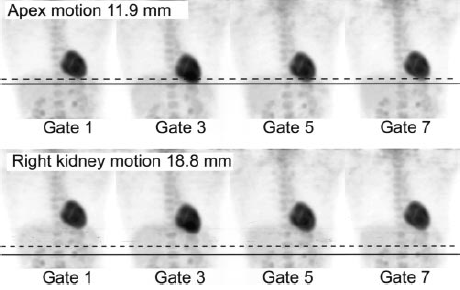
\includegraphics[width=12cm]{images/gatingBoucher2004}
	\end{center}
	\caption{Illustration de l'étendue du mouvement respiratoire sur des images reconstruites après synchronisation respiratoire~\cite{boucher2004respiratory}. La rangée du haut montre l'étendue du mouvement de l'apex du coeur, et celle du bas l'étendue du mouvement du rein} 
	\label{fig:boucher2004}
\end{figure}

Une variante de cette technique ne nécessitant pas de capteur est décrite dans~\cite{nehmeh2003reduction}. Un point faiblement radioactif est fixé au-dessus du torse du patient. Les acquisitions de l'imageur sont ensuite enregistrées par blocs temporels de 1 seconde, et une zone d'intérêt est reconstruite dans chacune des images. Les données reconstruites montrant le point source dans cette zone d'intérêt sont sommées et l'image finale reconstruite. 

Cette technique a été comparée avec celle présentée précédemment basée sur le système RPM. Ces deux techniques n'ont été testées cliniquement que sur un patient mais ont montrés des performances tout à fait semblables (6\% de différence dans les activités et 2\% pour le volume de la lésion).

Cependant ces techniques n'utilisent pas une carte d'atténuation optimisée pour la position du cycle correspondant aux acquisitions TEP.  Guoping et al.~\cite{GuopingChang2010Implementation} réalisent la carte d'atténuation à partir d'une image TDM réalisée en respiration libre synchronisée, et reconstruisent les données TEP acquises lorsque l'amplitude respiratoire est proche de celle utilisée pour l'acquisition TDM (voir exemples figure \ref{fig:chang2010}. Les résultats présentés sur 13 patients (21 tumeurs) montrent une amélioration du rapport signal sur bruit pouvant aller de -3.4 à 81\% suivant les tumeurs, avec une amélioration moyenne de 26.3\%.

\begin{figure}[h!]
	\begin{center}
		\begin{tabular}{c c}
			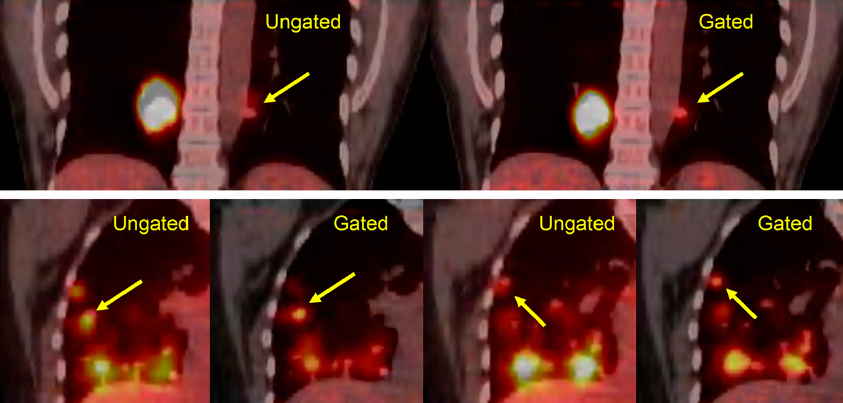
\includegraphics[width=10cm]{images/chang2010}
		\end{tabular}
	\end{center}
	\caption{Images TEP/TDM superposées du poumon reconstruites avec et sans gating respiratoire en utilisant la méthode décrite dans~\cite{GuopingChang2010Implementation}. On peut observer que les tumeurs sont mieux définies et correspondent à l'image TDM qui sert de référence.} 
	\label{fig:chang2010}
\end{figure}

Le principal problème de ces techniques est qu'elles demandent un temps d'acquisition beaucoup plus long à qualité d'image égale. Si l'on ne conserve que 20\% des évènements détectés, cela signifie qu'il faut augmenter le temps d'acquisition d'un facteur 5 pour obtenir une image d'une qualité égale. Il n'est donc pas envisageable de mettre en place ces protocoles en routine clinique, car le temps disponible n'est pas suffisant. C'est pour cela que de nombreuses équipes se sont mises à travailler sur une évolution de cette technique, où les images sont déformées les unes sur les autres pour prendre en compte toutes les informations de l'acquisition.

\section{Synchronisation respiratoire avec recalage}
\label{lab:corrPostRecon}

Dans cette section, nous allons détailler la technique consistant à corriger  le mouvement en déformant les images reconstruites.

Pour réaliser cela, les différentes techniques se basent sur une estimation préalable du mouvement respiratoire. Les images de chaque phase sont reconstruites indépendamment, puis recalées sur une phase de référence grâce au champ de mouvement. Enfin, les images déformées sont sommées. La difficulté se situe dans l'estimation du champ de mouvement interne lors de la respiration, car ce mouvement est complexe.

Les premières publications décrivant cette technique l'utilisaient notamment pour réaliser de l'imagerie cardiaque en TEP~\cite{klein19973d}. Cette publication démontre la faisabilité du procédé sur un animal en utilisant des techniques de flux optique pour estimer le champ de mouvement. En effet le coeur a l'avantage d'avoir une activité métabolique intense, ce qui rend l'estimation de son mouvement aisée même sur des images avec une faible statistique.

\subsection{Estimation du mouvement respiratoire corps entier}

L'estimation du champ de mouvement interne se fait à l'aide d'une des techniques présentées précédemment en \ref{lab:estimChamp}. Elles sont rappelées brièvement :

\subsubsection{imagerie TEP avec gating}
\label{lab:correctionDawood2008}

L`'acquisition TEP est réalisée en même temps que le signale respiratoire. Une image est reconstruite par phase du signal respiratoire, puis un algorithme d'estimation de mouvement est utilisé pour calculer le champ de mouvement entre les instants du cycle.

Les premiers algorithmes étaient utilisés en imagerie cardiaque~\cite{klein2002four} avec des transformations simples (affines), puis d'autres algorithmes plus adaptés aux images corps entier ont été utilisées, comme les flux optiques~\cite{dawood2006lung, dawood2006lung}, ou l'interpolation par B-spline~\cite{bai2009regularized}. 


\subsubsection{imagerie CT 4D}

Les images CT 4D peuvent être utilisées pour réaliser l'estimation du mouvement respiratoire au lieu des données TEP. Cela nécessite par contre une dose plus importante et un temps d'acquisition plus long.
Dawood a réalisé plusieurs publications sur le sujet en utilisant le flux optique pour l'estimation du champ de mouvement~\cite{dawood2006lung, dawood2008respiratory}. L'algorithme a été étudié sur des images de patients réels. Une autre publication~\cite{thorndyke2006reducing} indique une amélioration du rapport de contraste sur bruit (CNR) d'un facteur 3 grâce à la correction.


\section{Correction pré-reconstruction}

Les méthodes de correction du mouvement pré-reconstruction modifient les positions des Lignes de réponse (LDR) fournies par le scanner.
Ce recalage des LDR correspond à un déplacement des lignes de réponse dans l'espace du détecteur (voir fig. \ref{fig:recalageLOR}) en fonction du mouvement respiratoire. La limitation principale de ce type de méthode est que le champ de mouvement ne peut pas être élastique.

Cependant, il a été étudié en imagerie du cerveau~\cite{bloomfield2003design}, où il permettait de corriger les mouvements de la tête. Il a été aussi utilisé en imagerie cardiaque TEP~\cite{livieratos2005rigid} en utilisant un champ de mouvement rigide (rotation suivie d'une translation).

Dans les deux cas, les résultats ont montrés une nette amélioration des images (voir fig. \ref{fig:ameliorationLOR}

Dans le cadre du mouvement respiratoire du thorax, l'approche de recalage par LDR a été expérimentée par Frédéric Lamare~\cite{lamare2007respiratory}, mais avec des résultats mitigés.

\begin{figure}[h!]
	\begin{center}
		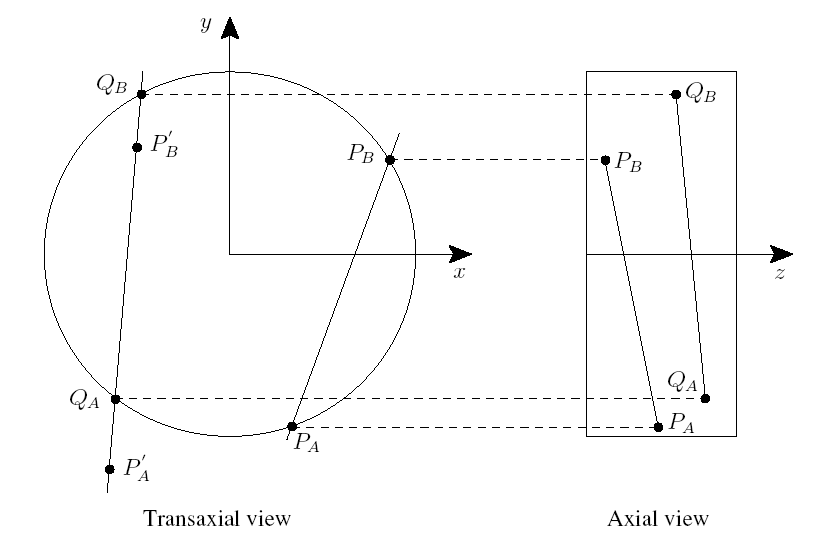
\includegraphics[width=12cm]{images/recalageLOR}
	\end{center}
	\caption{Illustration du recalage des lignes de réponse dans l'espace du détecteur : $P_A$ et $P_B$ représentent les positions des détections, $P_{A'}$ et $P_{B'}$ les positions des points corrigé et $Q_A$ et $Q_B$ les détections correspondantes } 
	\label{fig:recalageLOR}
\end{figure}

\begin{figure}[h!]
	\begin{center}
		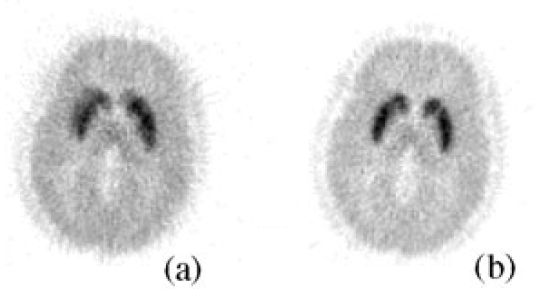
\includegraphics[width=6cm]{images/bloomfield2003design} 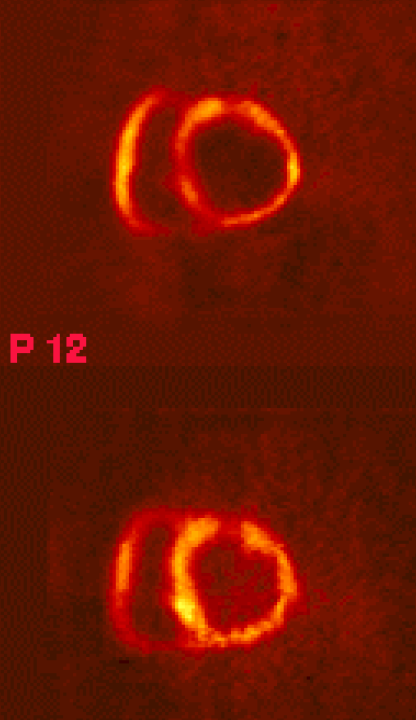
\includegraphics[width=3cm]{images/livieratos2005rigid}
	\end{center}
	\caption{Résultats de l'algorithme de recalage des LOR sur des images de patients utilisant le radio-traceur [$^{11}$C]raclopride. (a) montre une image non corrigée du mouvement et (b) une image corrigée. On peut noter que les éléments internes du cerveau sont beaucoup mieux définis. (c) représente une coupe du coeur petit axe non corrigée (en haut) et corrigée (en bas). On peut voir une amélioration de la définition de l'image.} 
	\label{fig:ameliorationLOR}
\end{figure}
 
Cette technique de correction du mouvement a été utilisée pour la correction du mouvement respiratoire du thorax~\cite{lamare2007respiratory,lamare2007list}, avec des performances plus limitées. En effet, le champ était approximé par une transformation affine, qui peut difficilement modéliser le mouvement du thorax dans son ensemble.

En effet, \cite{lamare2007respiratory} réalise une estimation du mouvement affine, en recalant les images TDM de chaque instant du cycle sur l'image de référence à l'aide d'une transformation affine par maximisation de l'information mutuelle normalisée. Le champ de mouvement  est calculé séparément pour le poumon, le coeur et trois organes sous le diaphragme (foie, estomac, rate). Les données sont des simulations réalisées par Geant4~\cite{jan2004gate} pour simuler un imageur Philips Allegro.

Ces résultats ont été améliorés par l'utilisation de la technique suivante qui permettait la prise en compte d'un mouvement élastique.

\section{Correction pendant la reconstruction}
\label{lab:CorrpendantRecon}
Plusieurs auteurs ont présentés des méthodes permettant de réaliser la correction de mouvement pendant la reconstruction. Qiao et al.\cite{qiao2006motion} et Lamare et al.~\cite{lamare2007list} ont proposé une méthode de correction du mouvement respiratoire basé sur une modification de la matrice de sensibilité lors de la reconstruction pour prendre en compte le mouvement. Tous les deux utilisent un champ de mouvement élastique estimé en utilisant un champ interpolé par B-splines.

L'algorithme original utilisé est basé sur OPL-EM~\cite{reader2002one} qui organise les données en ``sous-ensemble'' de la même manière que OS-EM~\cite{hudson1994accelerated} mais en utilisant les informations list-mode. Le principe de la reconstruction avec correction du mouvement respiratoire est décrit par la formule suivante :

\label{lab:corrMatSyst}
\begin{equation}
 f^{k+1}=\frac{f^k}{S} \sum_{t=1}^{N_{frames}} P_t^T \frac{1}{P_t f^k} 
\end{equation}

$f^k$ est l'image à l'itération $k$,

$T$ est l'opérateur de transposition

$P_t$ représente la matrice système à l'instant t. Chaque élément $p_{ij}$ de cette matrice indique la probabilité de détecter à la ligne de réponse $i$ un évènement généré au voxel $j$. 

$N$ correspond au nombre d'instants temporels considérés.

$S$ est la matrice de sensibilité :

\begin{equation}
 S=\frac{1}{N_{frames}} \sum_{t=1}^{N_{frames}} P_t^T N A_t 
\end{equation}

 $A_t$ est la matrice permettant de corriger les effets de l'atténuation au temps $t$ et $N$ est la matrice de normalisation qui compense l'inhomogénéité spatiale de la sensibilité.

Dans la publication~\cite{lamare2007list}, deux variantes de cette technique sont comparées avec la correction par synchronisation respiratoire avec recalage présentée précédemment ainsi que la correction pré-reconstruction. Les résultats présentés montrent un clair avantage pour la correction pendant la reconstruction, avec des performances couramment améliorées d'un facteur 2. 

Par exemple, la différence relative du contraste (équation \ref{eq:percentAmelioraiton}) pour une lésion de 7mm présente dans la partie haute du poumon est de 28\% pour les images non corrigées, contre 4.4\% pour les images corrigées par la méthode de correction pré-reconstruction et de 1.2\% pour la méthode de reconstruction pendant la reconstruction. De la même manière, pour des lésions de 7mm présentes dans le bas du poumon, les images non corrigées montrent une différence relative de contraste de 32\%, contre 2.63\% pour la correction pré-reconstruction et 1.66\% pour la correction pendant la reconstruction.


\begin{equation}
 \label{eq:percentAmelioraiton}
 \% Am\acute{e}lioration = \left| \frac{Image~\acute{E}valu\acute{e}e~-~R\acute{e}f\acute{e}rence}{R\acute{e}f\acute{e}rence} \right|
\end{equation}

La figure \ref{fig:lamare2007} montre un profil de l'interface poumon/foie avec une tumeur pour les différentes techniques de correction. On voit clairement que l'image non corrigée montre un retard dû au flou de mouvement. Ce retard est partiellement corrigé par la correction de mouvement pré-reconstruction, mais le profil de courbe de la méthode de correction du mouvement pendant la reconstruction est celui qui s'approche le plus de la référence.


\begin{figure}[h!]
	\begin{center}
		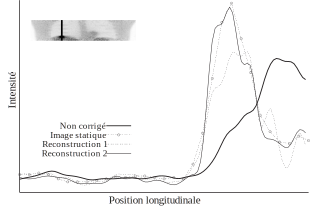
\includegraphics[width=12cm]{images/lamare2007list}
	\end{center}
	\caption{comparaison des performances des différentes techniques de correction du mouvement sur un profil d'image TEP contenant une tumeur placée au niveau du diaphragme. La référence correspond à Frame 1, LORs-Affine correspond à la correction pré-reconstruction et Elastic Method 2 corresponds à la correction pendant la reconstruction.} 
	\label{fig:lamare2007}
\end{figure}


\section{Déconvolution de l'image}

Cette technique décrite en ~\cite{naqa2006deblurring} utilise une connaissance du mouvement respiratoire acquise à partir d'une image TDM 4D pour déduire un filtrage appelé TLP (\textit{Tumor Location Probability}) qui correspond à la dégradation dû au mouvement respiratoire.

L'image est ensuite déconvoluée pour corriger les effets du mouvement respiratoire. Cette méthode a été évaluée sur un fantôme physique et des patients réels à l'aide d'un grand nombre de critères provenant pour partie de la TEP (sous-estimation de l'activité de la tumeur, exemples d'images), et pour partie du domaine de la déconvolution (entropie, ``rugosité'').

Les résultats présentés en \ref{fig:performanceDeconvolution} montrent une nette amélioration des performances sur des fantômes, pour un déplacement axial simple de 20mm. L'activité des lésions de fort diamètre est correctement récupérée quelque soit l'algorithme utilisée, mais il n'a pratiquement pas d'effets sur les lésions de 1cm de diamètre.

Ce type d'algorithme est peu présenté dans la littérature. 

\begin{figure}[h!]
	\begin{center}
		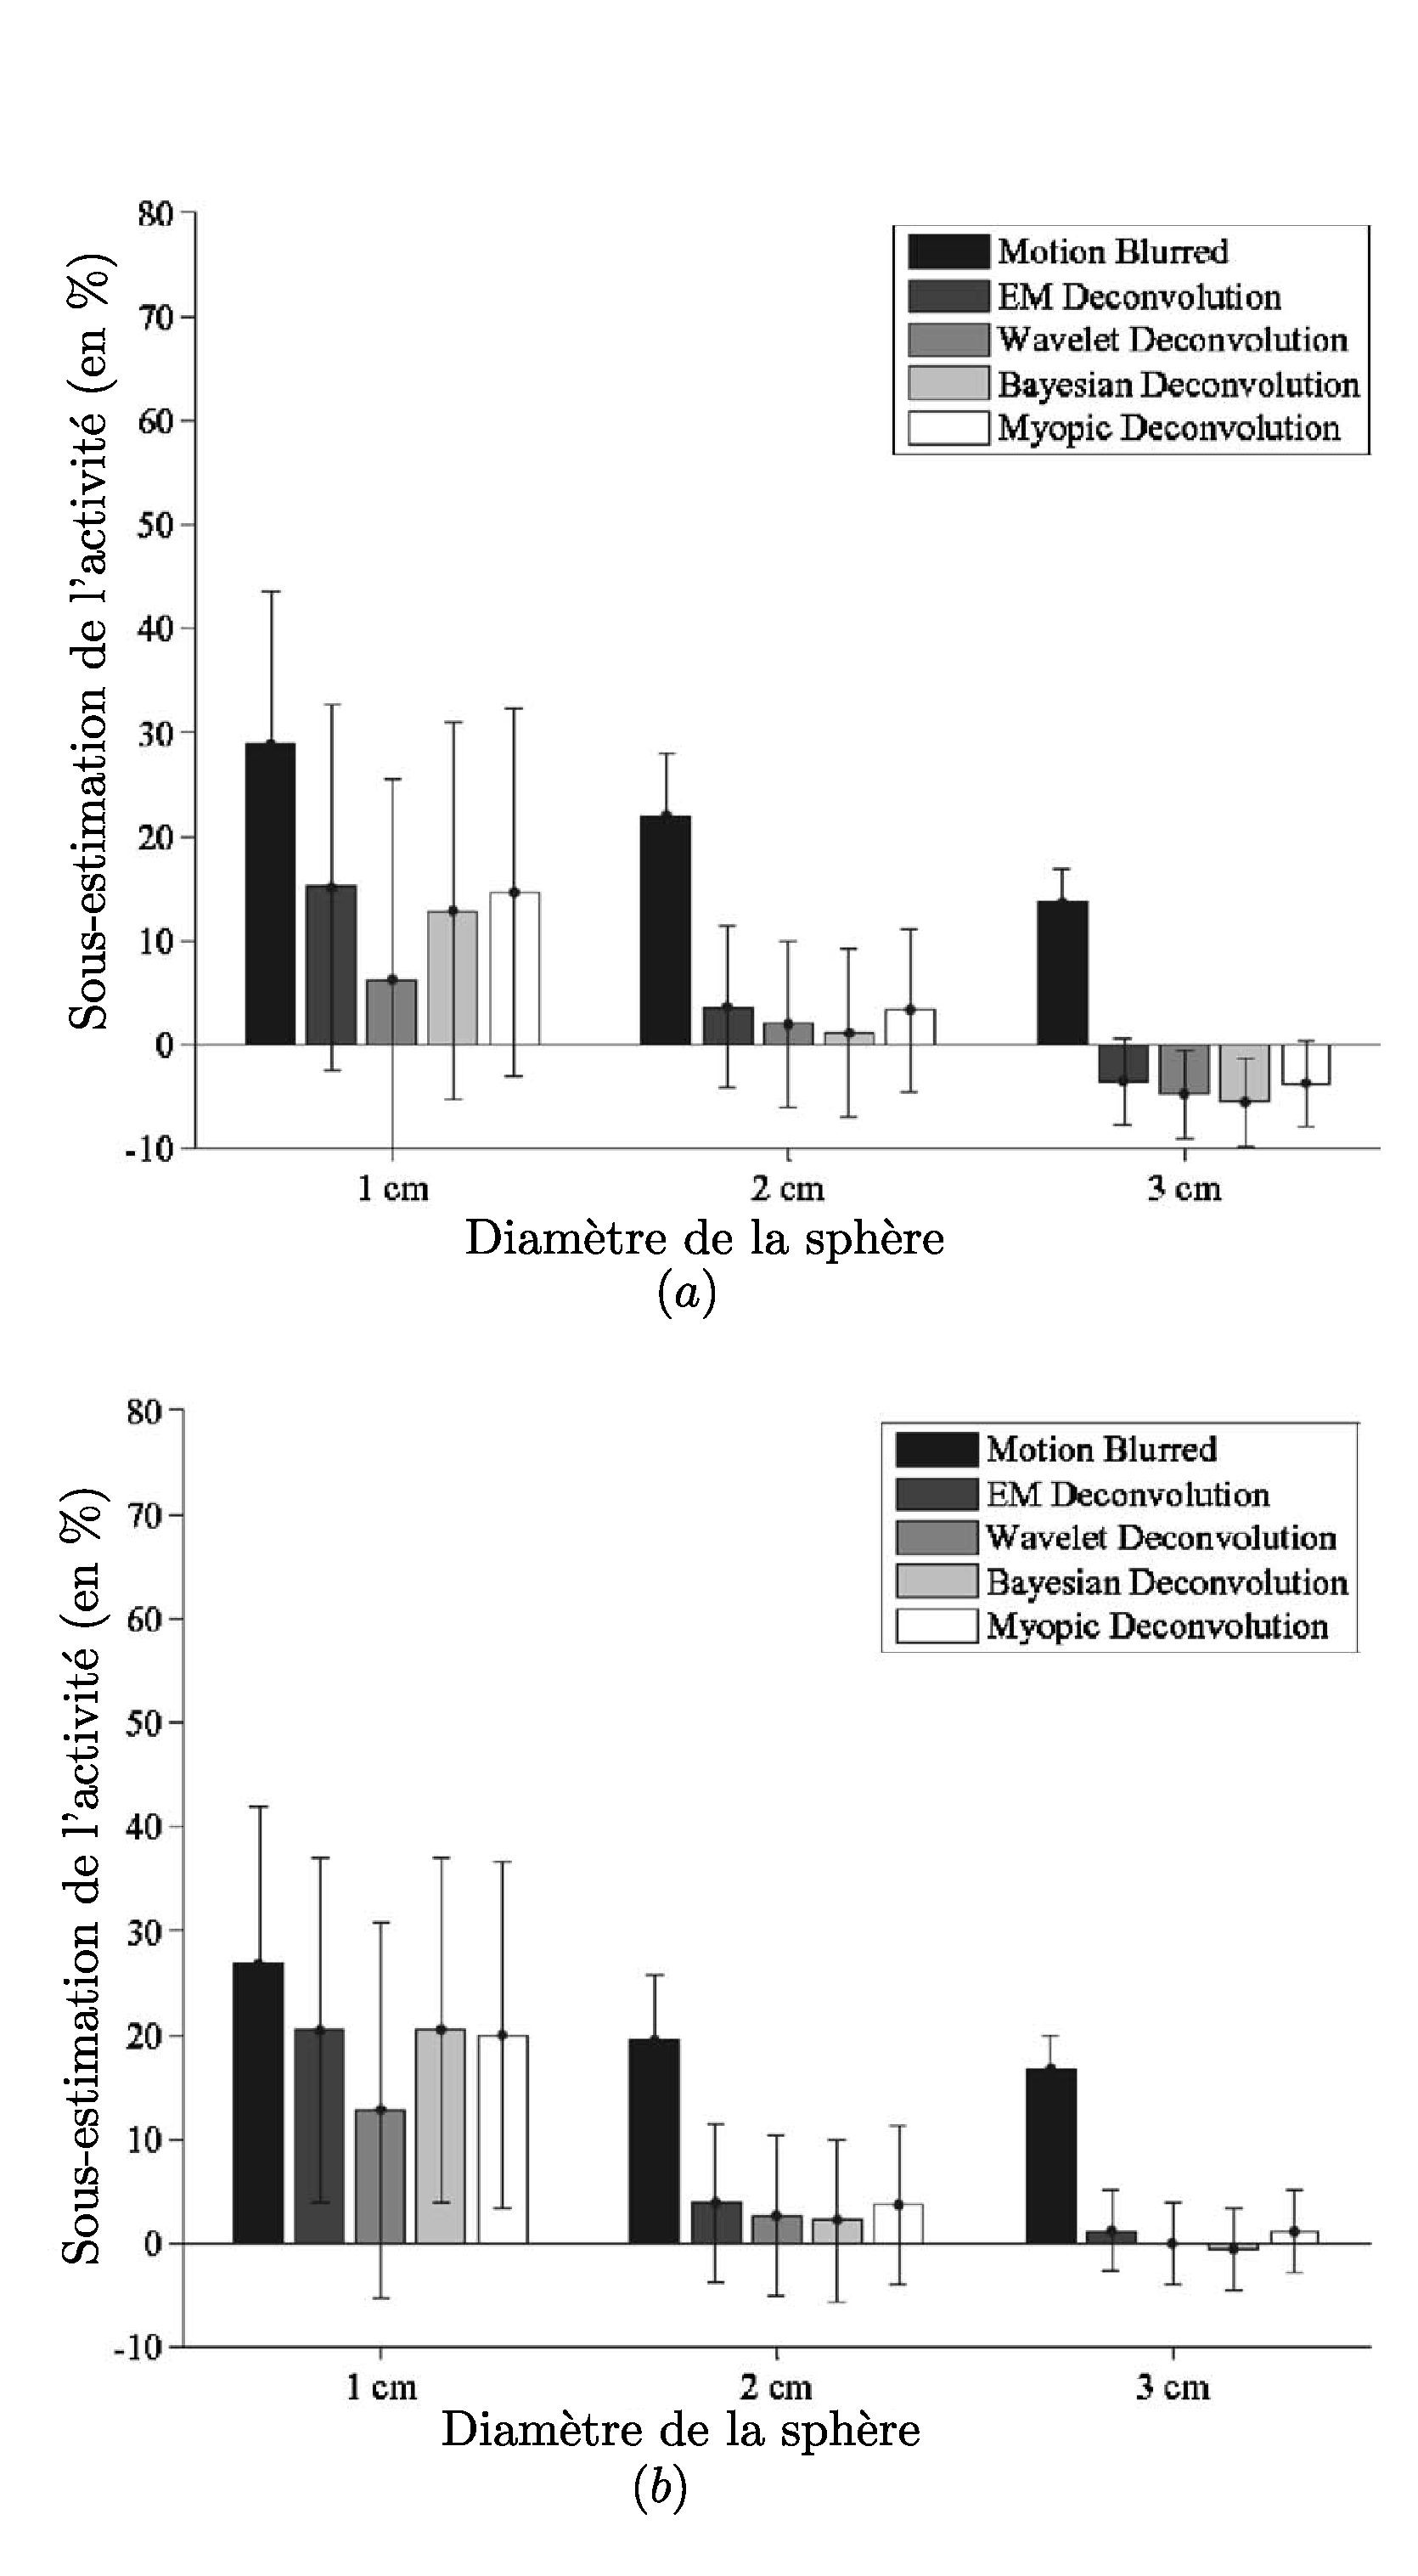
\includegraphics[width=10cm]{images/performanceDeconvolution}
	\end{center}
	\caption{Comparaison de l'erreur de sous-estimation de l'activité des lésions en fonction de l'algorithme de déconvolution utilisé sur des fantômes. En a) la lésion a une activité moyenne, tandis qu'en b) l'activité de la lésion est faible par rapport au fond. Le déplacement de la lésion est le même dans les deux cas (2cm)} 
	\label{fig:performanceDeconvolution}
\end{figure}


Un autre article utilisant aussi des algorithmes de déconvolution a été présenté par wiemker~\cite{wiemker2008combined}. Cependant il ne cherche pas à corriger le mouvement respiratoire sur l'ensemble de l'image mais principalement à améliorer la mesure du SUV sur une lésion. Pour cela, il réalise une estimation de la fonction d'étalement du point (FEP) de l'imageur TEP au niveau de la lésion à l'aide d'un contourage de la lésion réalisé préalablement dur une image TDM. L'estimation de la FEP permet de prendre en compte à la fois les effets du mouvement respiratoire et ceux de la FEP intrinsèque à l'imageur TEP. 

Cependant, cette technique est inapplicable dans notre cas car les lésions doivent être suffisamment importantes et homogènes pour pouvoir les délimiter de manière fiable sur les images TDM, ce qui n'est pas notre cas.


\part{Evaluation des performances de diagnostique}
	\chapter{Problématique de la détection}
		\section{Historique}
		\section{courbes ROC}
		\section{Free-ROC}	
	
	\chapter{Systèmes de détection}
		\section{Les CAD en TEP}
		\section{Types de classification}
			\subsection{supervisée - méthodologie}
			\subsection{non supervisée - méthodologie}
		\section{classifieurs}
			\subsection{SVM}
			\subsection{LDA}
		\section{Systèmes humain}
		% besoin d'avoir des données fiables ?


\part{Simulation et base de données (MIC 2011)}
	\chapter{Simulations}
		\section{principe des simulations}
			\subsection{monte carlo}
			\subsection{analytiques}
			\subsection{MC accélérés}

		\section{simulateurs disponibles}
		\section{processus de simulation avec SORTEO}
		\section{Contribution à SORTEO}

	\chapter{Base de donnée}
		\section{Présentation}
		\section{Modèles}
		\section{données clef} % temps de calculs etc....


\part{Résultats}
	\chapter{méthodes (MIC 2010)}
        \chapter{analyse critique des résultats}

\part{Conclusion}




\part{Bibliographie}
\bibliographystyle{apalike}
\bibliography{biblio}

\end{document}

